\section{Analysis 1b}
	\subsection{Differentialrechnung S. 444 ff}

				\begin{tabular}{llll} 
				Kurvenuntersuchungen & S. 261 & Taylor-reihe & S. 455 \\
				\end{tabular}
				
				
			\subsubsection{Begriff der Ableitung / Differenzialquotient S. 444}
			Die Ableitung $f'(x)$ der Funktion $f(x)$ im Punkt $x_0$ entspricht der Steigung der Tangente an	$f(x)$ im Punkt $x_0$		 \\
			\\
			\begin{tabular}{ll}
			Differenzenquotient: & $\frac{f(x + h) - f(x)}{h} = \frac{f(x + \Delta x) - f(x)}{\Delta x}$ \\
			\\
			\textbf{Differenzialquotient:} & $f'(x) = \lim\limits_{\Delta x \to 0} \frac{f(x + \Delta x) - f(x)}{\Delta x}$ \quad $(\Delta x = h)$ \\
			\end{tabular}
			

			\subsubsection{Tangente / Normale / Zwischenwinkel}
			\begin{tabular}{ll}
			Tangente: & $y = f'(x_0) \cdot (x - x_0) + y_0$ \\
			\\
			Normale: & $y = -\frac{1}{f'(x_0)} \cdot (x - x_0) + y_0$ \\	
			\\
			Zwischenwinkel: &  $tan(\alpha) = \frac{m_1 - m_2}{1 + m_1 \cdot m_2} \rightarrow$ Winkel gegen Uhrz.\\
			\\
			&  $tan(\alpha) =  \frac{m_2 - m_1}{1 + m_1 \cdot m_2} \rightarrow$ Winkel im Uhrzeigersinn\\
			
			\end{tabular}
			
			
			\subsubsection{Einseitige Ableitungen S. 445}
			rechtsseitig: $f'_r(x_0) = \lim\limits_{x \to x_0^+}f'(x)$ \quad
			linksseitig: $f'_l(x_0) = \lim\limits_{x \to x_0^-}f'(x)$ \\
			\\
			\begin{tabular}{ll}
			$f'_r(x_0) = f'_l(x_0)$ & $\rightarrow$ Konvergenz \\
			Alle anderen Fälle & $\rightarrow$ unbestimmte Divergenz $\rightarrow$ keine Ableitung! \\
			\end{tabular}
			
			

		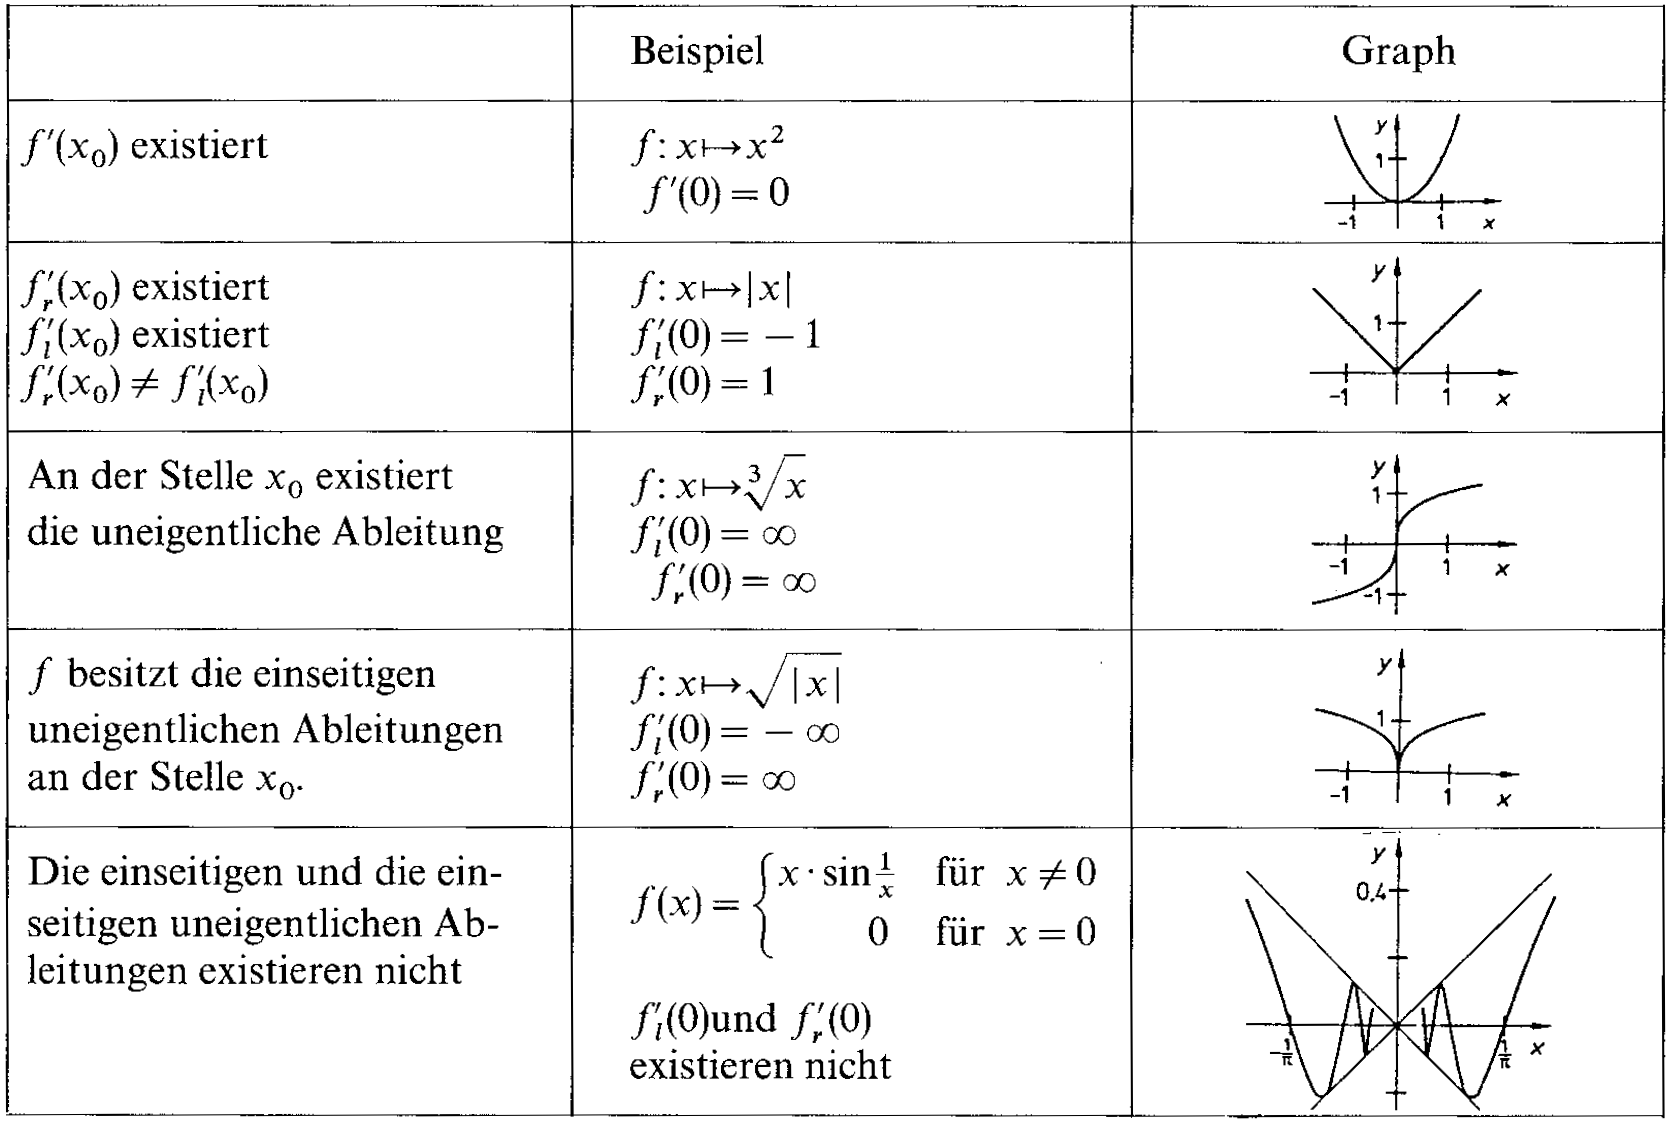
\includegraphics[width=0.9\linewidth]{Bilder/konvergenz-divergenz}
			
			
			\subsubsection{Generische Muster}
			\begin{tabular}{ll}
			Allg. Potenz &  $\left( f(x)^\alpha \right)' = f'(x) \cdot \alpha \cdot f(x) ^{\alpha - 1} $ \\
			\\
			Allg. log-Regel & $\ln \left( f(x) \right)' = \frac{f'(x)}{f(x)} $ \\
			\\
			Allg. exp-Regel & $ \left( \e^{f(x)} \right)' = f'(x) \cdot \e^{f(x)} $ \\
			\end{tabular}
			
			
			\subsubsection{Ableitungsregeln S. 445-448}
			
			\textbf{Elementare Regeln}\\
			\begin{tabular}{lll}
			Potenzen: & $f(x) = x^3$ & $f'(x) = 3 \, x^2$ \\
			& $f(x) = x^\alpha$ & $f'(x) = \alpha \cdot x^{\alpha - 1}$ \\
			\\
			Linearität: & $f(x) = c \cdot x^2$ & $f'(x) = c \cdot 2 \, x $ \\
			\\
			Summe: & $(u(x) + v(x) - w(x))' $ & = $u'(x) + v'(x) - w'(x)$ \\
			\\
			Konstanten: & c = konst $\rightarrow$ c' = 0 \\
			\end{tabular}
			
			
			\textbf{Produktregel}\\
			$(f(x) \cdot g(x))' = f'(x) \cdot g(x) + f(x) \cdot g'(x)$ 
			
			\textbf{Quotientenregel}\\
			$\left( \frac{u(x)}{v(x)} \right) ' = \frac{u'(x) \cdot v(x) - u(x) \cdot v'(x)}{v(x) ^2}$ \quad $\rightarrow$ als Produkt schreiben \\
			\\
			$u(x) \cdot \left( \frac{1)}{v(x)} \right) ' =  u'(x) \cdot \frac{1}{v(x)} + u(x) \cdot \frac{- v'(x)}{v(x)^2}$
			
			\textbf{Kettenregel}\\
			$g(f(x))' =  f'(x) \cdot g'(x)$ \\
			
			\textbf{Umkehrfunktion}\\
			$(f^{-1}(y_0))' = \frac{1}{f'(x_0)} =  \frac{1}{f'(f^{-1}(y_0))}$ \\
			

			
			\subsubsection{Allgemeine Logarithmus-Ableitung}
			$(\log_b(x))' = \left( \frac{\ln(x)}{\ln(b)} \right)' = \frac{1}{\ln(b)} \cdot (\ln(x))' = \frac{1}{\ln(b)} \cdot \frac{1}{x} $
			
			
			\subsubsection{Lineare Approximation / Differenzial dy S. 459}
			Differenzial = dy = df = "Höhenunterschied der Tangente" \\
			= "Linearzuwachs" \\
			\textcolor{blue}{Differenzial = $f'(x_0) \cdot dx$} $= f'(x_0) \cdot h = f'(x_0) \cdot \Delta x = f'(x_0) \cdot (x- x_0) $ \\
			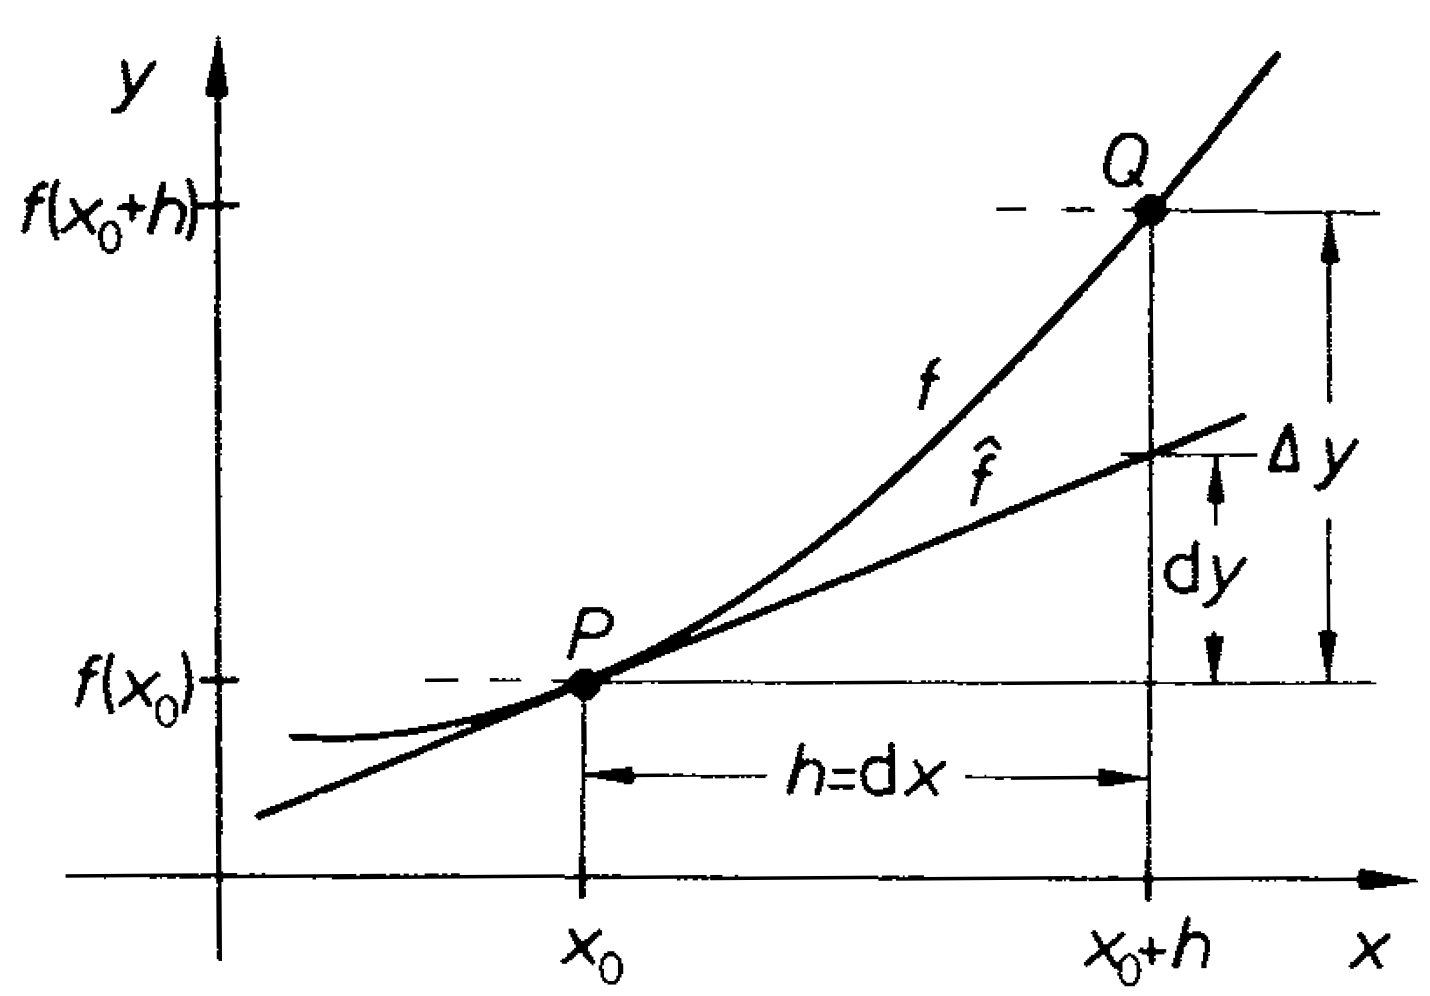
\includegraphics[width=0.8\linewidth]{Bilder/differenzial}  \\
			$\Delta y \approx dy \rightarrow$ Approximation / Fehler \\
			Fehler : \quad $\Delta y - dy \rightarrow 0$ \quad $h \rightarrow 0$ \\	
			Tangentengleichung: $\hat f(x): y_0 + f'(x_0) \cdot (x - x_0)$ \\
			\textbf{Die Tangente ist die beste lineare Approximation!}		
			
			
			\subsubsection{Approximationsfehler}
			Die Fehler beziehen sich auf den Arbeitspunkt (z.B. $x_0$) \\
			\\
			\begin{tabular}{lll}
			Absoluter Fehler: & $\Delta y - dy = f(x) - \hat f(x)$ & Einheit y \\
			\\
			Relativer Fehler: & $\frac{\Delta y - dy}{y_0} = \frac{f(x) - \hat f(x)}{x_0} $ & Einheitenlos \\
			\end{tabular}
			
			
			\subsubsection{Fehlerfortpflanzung} 
			\begin{tabular}{llll}
			Absolut: & $\Delta x \rightarrow \Delta y$ & &
			$\Delta y \approx dy = f'(x_0) \cdot dx$ \\
			\\
			Relativ: & $\Delta x \rightarrow \frac{\Delta y}  {y_0}$ & &  $\frac{\Delta y}  {y_0} \approx \frac{dy}{y_0} = \frac{f'(x_0) \cdot dx}{y_0} $ \\
			\end{tabular}
			 \\

			\begin{tabular}{| c | c | c |}
			\hline
			& $\Delta x = dx$ (abs) & $\frac{\Delta x}{x} = \frac{dx}{x}$ (rel)  \\
			\hline
			$\Delta y \approx dy$ (abs) & A & B \\
			\hline
			$\frac{\Delta y}{y} \approx \frac{dy}{y}$ (rel) & C & D \\
			\hline
			\end{tabular}					
			\\ \\
			$\rightarrow$ Tabelle ist bidirektional (Umkehrfunktionen)
			
			
			\subsubsection{Wichtige Ableitungen S.446}
			
			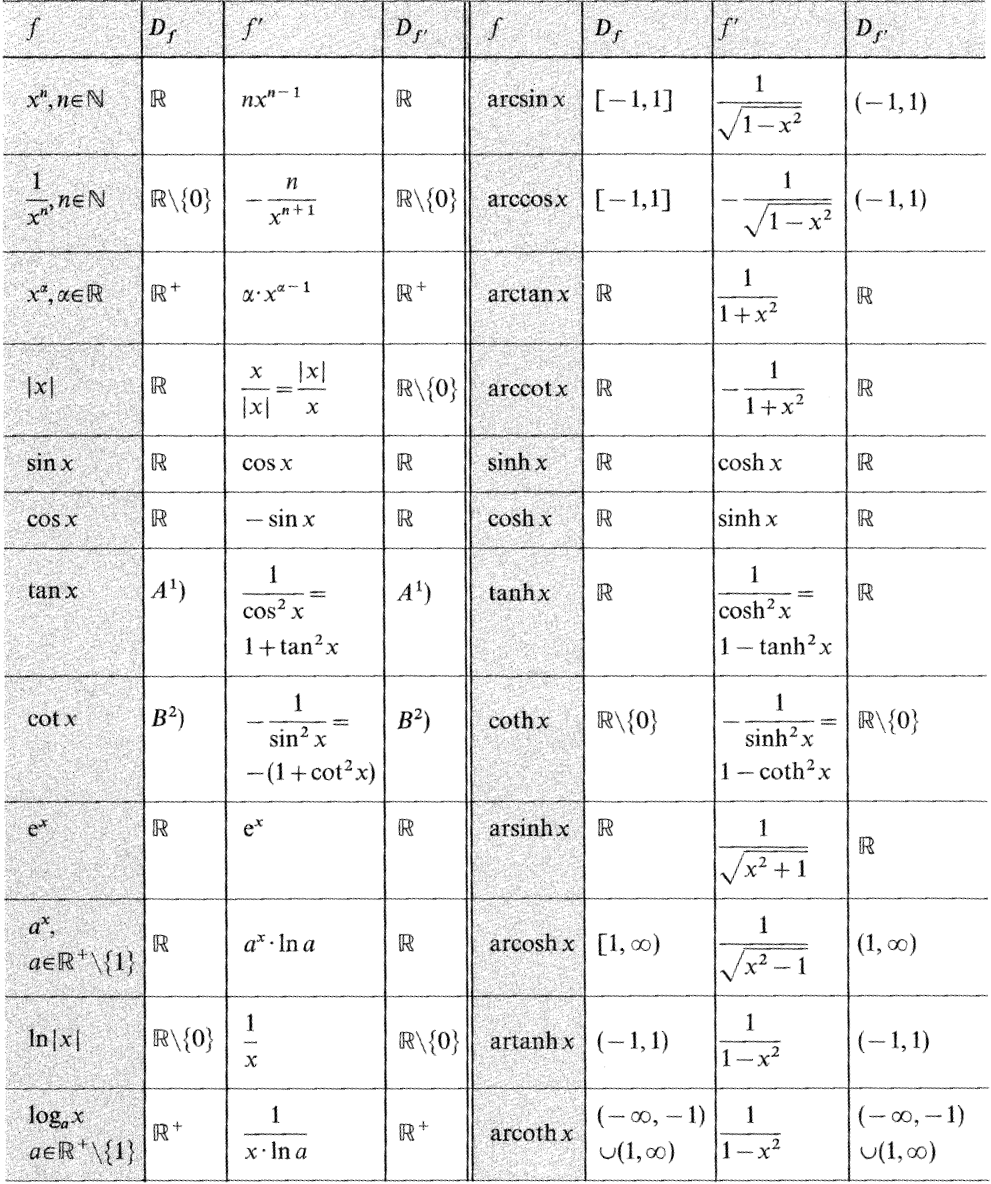
\includegraphics[width=\linewidth]{Bilder/ableitungen}

			
			\subsubsection{Taylor-Reihe (Approximation höherer Ordnung)}
			n = Ordnung der Approximationsfunktion $p_n(x)$ \\
			$h = x - x_0$ \\
			\\
			$p_n(x) = f(x_0) + f'(x_0) \cdot h + \frac{f''(x_0)}{2!} \cdot h^2 + ... + \frac{f^{(n)}(x_0)}{n!} \cdot h^n$	 \\
			\\
			$p_n(x) = \sum\limits_{k=0}^{n} \frac{f^{(k)}(x_0)}{k!} \cdot h^k \; \vert h = x-x_0$\\
			\\
			Der Approximationsfehler $R_n (x_0, h)$ entspricht $f(x) - p_n(x)$ und wird im nächsten Abschnitt beschrieben.		
			
			
			\subsubsection{Fehler $R_n$ der Taylor-Reihe}
			Der Fehler ist nicht klar berechenbar, sondern nur auf einem Intervall "bestimmbar" $\rightarrow$ Worst Case! \\			
			Voraussetzung: f auf Intervall [a;b] mind. (n+1) mal ableitbar\\
			\\
			\begin{tabular}{ll}
			\textbf{Lagrange:} &  $\vert R_n \vert = \vert \frac{f^{(n+1)}(\xi)}{(n+1)!} \cdot h^{n+1} \vert $ \\
			\\
			\textbf{Cauchy:} & $\vert R_n \vert = \vert \frac{f^{(n+1)} (\xi)}{n!}  \cdot h^{n+1} \cdot (1 - \theta)^n \vert$ \\
			\\
			& $0 < \theta < 1$    $\xi = x_0 + \theta \cdot h$ \\
			& $\theta$ steuert Lage von $\xi$ auf Intervall \\
			\end{tabular}
			
		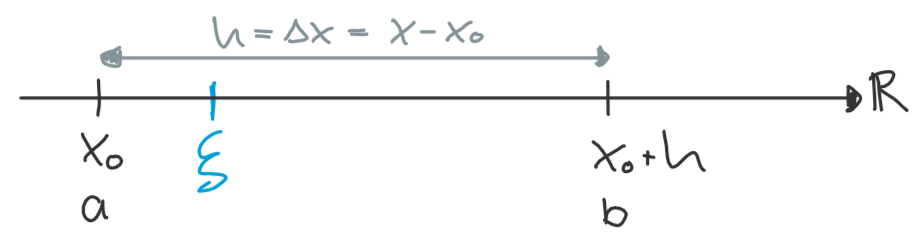
\includegraphics[width=0.7\linewidth]{Bilder/zahlenstrahl}
			
			
			\textbf{Verhalten von $R_n$}	\\
			
			\begin{tabular}{llll}
			1) & $n \rightarrow \infty$ & "Normal" \quad $R_n \rightarrow 0$ & $\vert h \vert$ fix  \\
			2) & $n \rightarrow 0^+$ & "Normal" \quad $R_n \rightarrow 0$ & n fix \\
			& &  $\vert f^{n+1}(\tilde{x})\vert < K^{n+1}$ & $(K < 0, n \in \mathbb{N}_0), \tilde{x} \in (a;b)$ \\
			\end{tabular}
			
			
			\subsubsection{Satz von Rolle S. 454}
			\begin{tabular}{ll}
			Voraussetzungen: & f auf Intervall [a;b] mind. (n+1) mal ableitbar\\
			 & $f(a) = f(b)$ \\
			\end{tabular}
			
			Auf dem Intervall (a;b) existiert mindestens einmal  eine horizontale Tangente : $f'(\xi) = 0$ \\			
			 \\
			 

			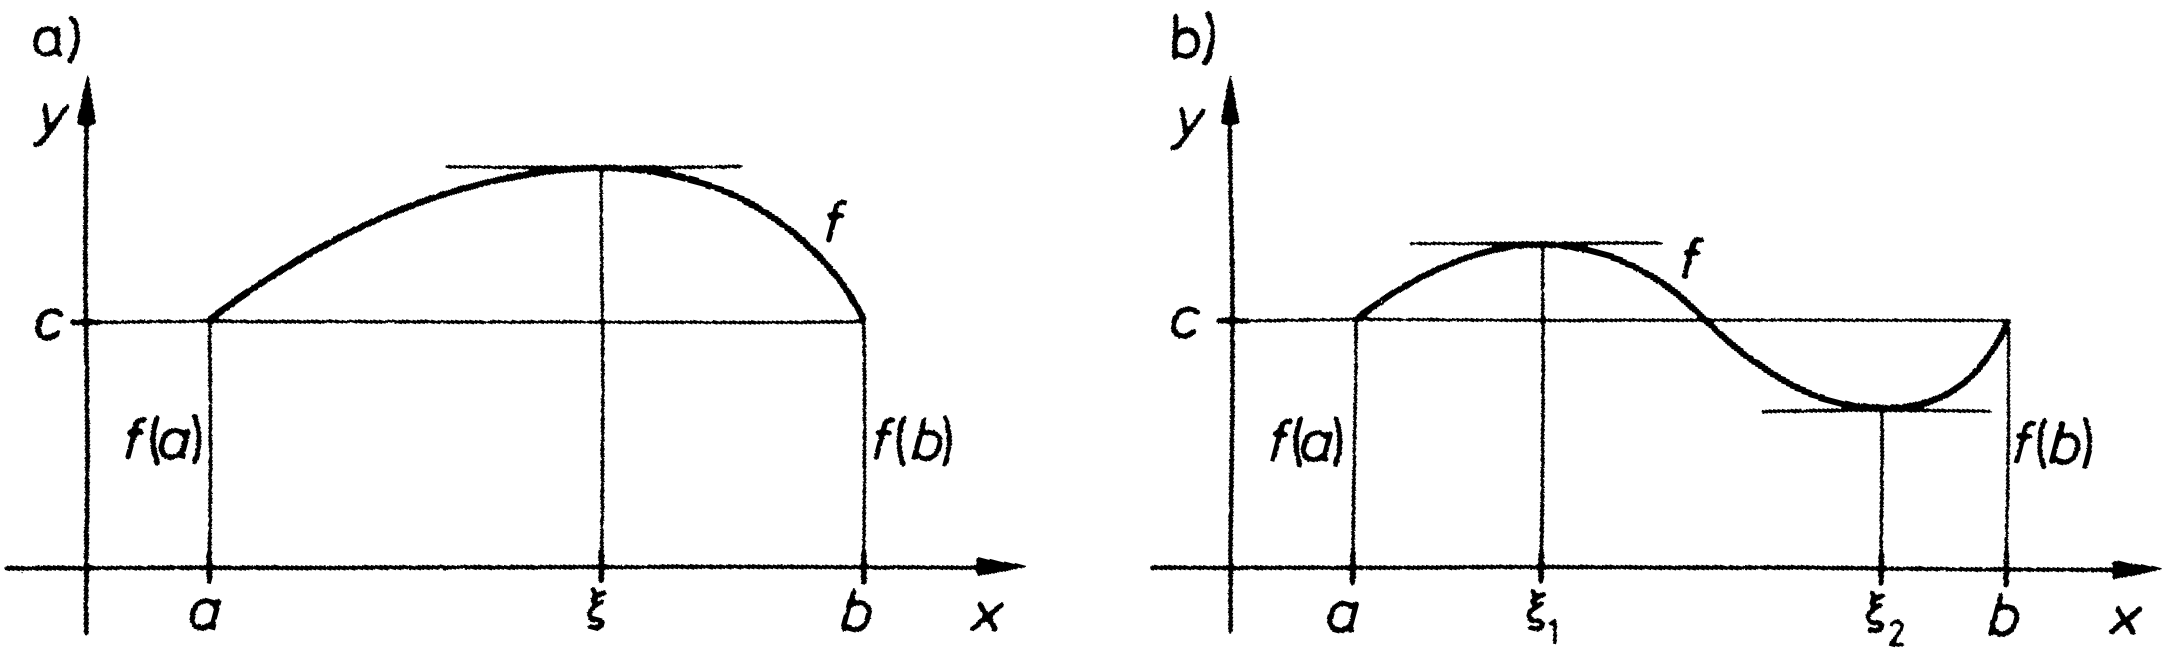
\includegraphics[width=0.9\linewidth]{Bilder/rolle}
			
			
			
			\subsubsection{Mittelwertsatz S. 454}			
			\begin{tabular}{ll}
			Voraussetzungen: &  f auf Intervall [a;b] mind. (n+1) mal ableitbar \\
			\end{tabular}

			\begin{minipage}[b]{.5\linewidth} 
  			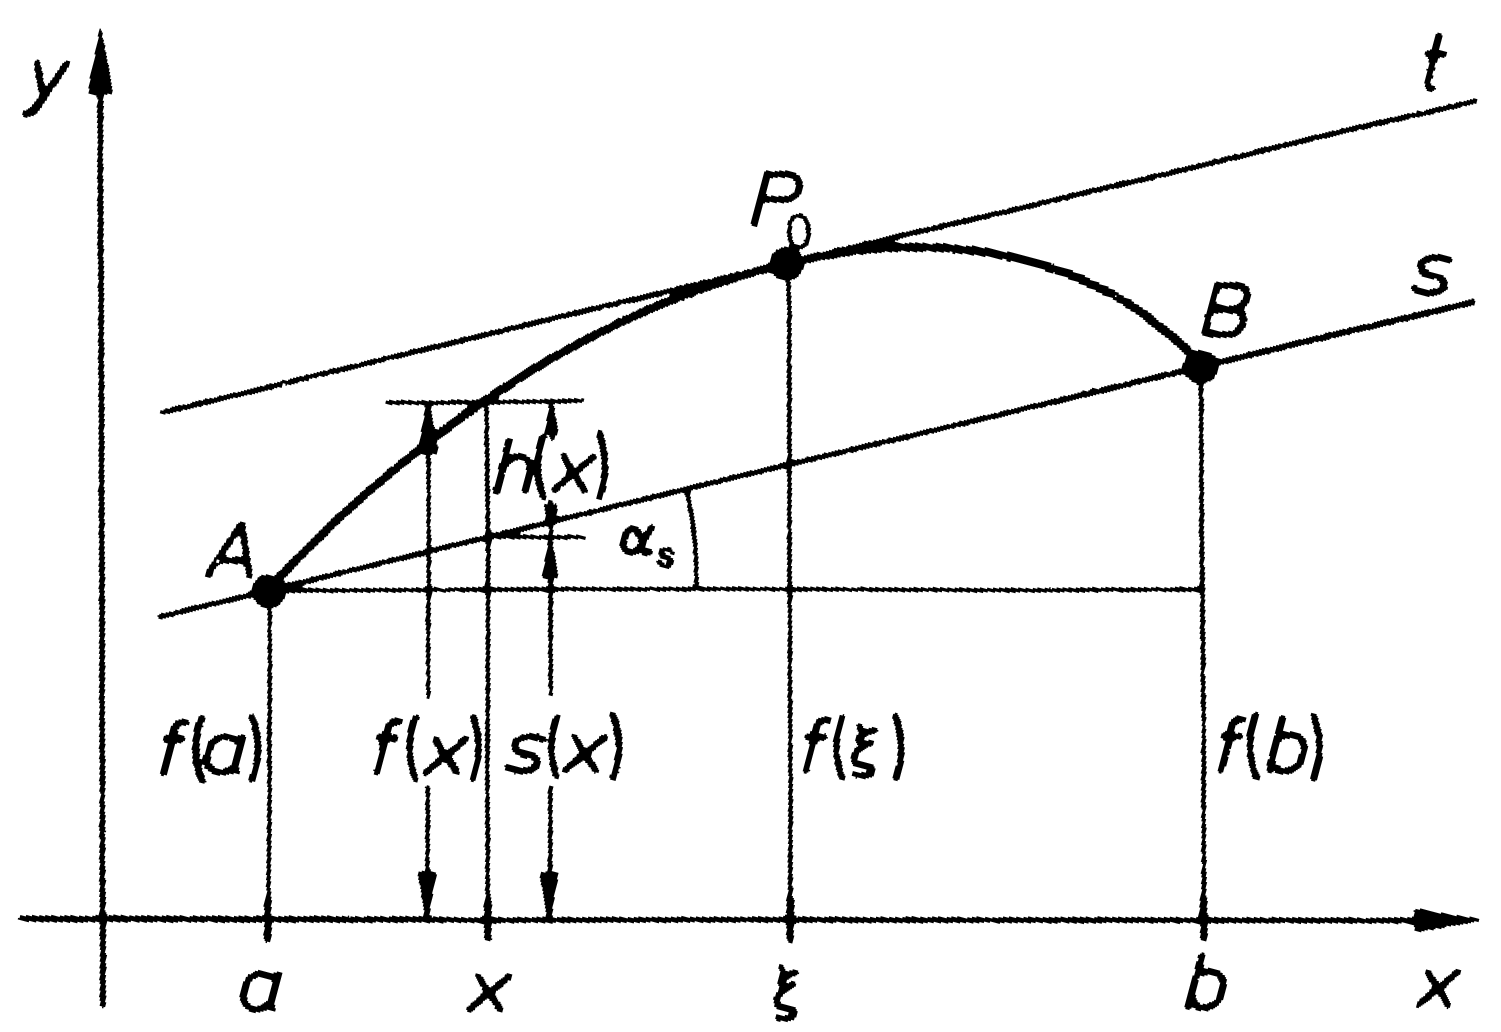
\includegraphics[width=\linewidth]{Bilder/mittelwertsatz}
			\end{minipage}
			\hfill
			\begin{minipage}[b]{.45\linewidth} 
  			
  			Sekantensteigung: \\
  			$m_s = \frac{\Delta y}{\Delta x} = \frac{f(b) - f(a)}{b - a}$ \\
  			\\
  			
  			Tangentensteigung / \\
  			Durchschnittssteigung:
  			$f'(\xi) = \frac{f(b) - f(a)}{b - a}$ \\		
				
			\end{minipage}			
		
			
			\subsubsection{Extremalstellen S. 455-457}
			f: [a;b] $\rightarrow$ $\mathbb{R}$ , stetig $\Rightarrow W_f$ = abgeschlossenes Intervall 
			
			\textbf{Absolut Extremalstelle (Randanalyse durchführen)}\\
			\begin{tabular}{ll}
			Absolutes Maximum: &  $\mathrm{max}(W_f)$\\
		  	Absolutes Minimum & $\mathrm{min}(W_f)$ \\
			\end{tabular}
			
			\textbf{Relative Extremalstelle}\\
		
			\begin{tabular}{ll}
			Lokales Maximum: & "Berg" (nicht am Rand der Funktion)\\ 
			& $f(x) \leq f(x_0) $ \quad $x \in U_{\delta}(x_0)$  \\
			&Wechsel von $\uparrow$ zu $\downarrow$ \\
			\\
			Lokales Minimum: & "Tal" (nicht am Rand der Funktion)\\
			& $f(x) \geq f(x_0) $ \quad $x \in U_{\delta}(x_0)$ \\
			& Wechsel von $\downarrow$ zu $\uparrow$ \\
			\\	
			Terrasse: & $f'(x_0) = 0$ aber kein "Berg" / "Tal" \\ 
			\end{tabular}
			
			
			\textbf{Prinzip von Fermat S. 453}	\\
			Wenn $x_0$ ein relatives Minimum / Maximum ist muss zwingend die Ableitung $f'(x_0) = 0$ sein	 $\rightarrow$ \textbf{Umkehrung gilt nicht!}\\
			$x_0$ = kritische Stelle $\rightarrow$ zu prüfen auf Berg, Tal oder Terrasse \\
			
			\begin{tabular}{| c | c | c | l |}
			\hline
			$f'(x_0)$ & $f''(x_0)$ & $f^{(n)}(x_0)$ & \\
			\hline
			0 & $< 0$ &  & "Berg" (Achtung auf Randstellen) \\
			\hline
			0 & $> 0$ & & "Tal" (Achtung auf Randstellen) \\
			\hline
			0 & 0 & $< 0$ & wenn n gerade: "Berg" \\
			\hline
			0 & 0 & $> 0$ & wenn n gerade: "Tal" \\
			\hline
			0 & 0 & $\neq 0$ & wenn n ungerade ; Terrasse \\
			\hline
			\end{tabular}
			
			\vspace{0.1cm}
			y-Koordinate des Punktes: $x_0$ in f(x) einsetzen					
			
			\subsubsection{Monotonie S. 453}
			\begin{tabular}{| c | l |}
			\hline
			$f'(x_0)$ &  \\
			\hline
			$ \geq 0$  & monoton wachsend \\
			\hline
			$ \leq 0$ & monoton fallend \\
			\hline
			$ > 0$  &  streng monoton wachsend \\
			\hline
			$ < 0$  &  streng monoton fallend \\
			\hline
			\end{tabular}
			
			
			\subsubsection{Wendepunkte (Terrassenpunkte)}
			Wendepunkt = Krümmungswechsel = Vorzeichenwechsel für $f''(x)$ bei $x_0$ \\
			
			\begin{tabular}{| c | c | c | l |}
			\hline
			$f'(x_0)$ & $f''(x_0)$ & $f^{(n)}(x_0)$ & \\
			\hline
			 & 0 & $ < 0$ & n ungerade: links-rechts Wendestelle \\
			\hline
			 & 0 & $ > 0$ & n ungerade: rechts-links Wendestelle \\
			\hline
			 & 0 & $\neq 0$ & n gerade: Flachpunkt \\
			\hline
			\end{tabular}
			
			Ausserdem liegt eine WP vor wenn $f''$ beim Durchgang durch $x_0$ das Vorzeichen wechselt, also $f''(x_0) < 0$ für $x < x_0$ und für $f''(x_0) > 0$ für $x > x_0$ bzw. umgekehrt.\\
			
			y-Koordinate des Punktes: $x_0$ in f(x) einsetzen		


			\subsubsection{Krümmungsverhalten} 
			Das beschriebene Verhalten gilt global für die ganze Funktion f(x) bzw. auf einem ganzen Intervall, nicht nur an einer Stelle $x_0$!
			
			\textbf{Linkskrümmung (konvex)}\\
			\begin{tabular}{ll}
			$\bullet$ & $f(x) \geq f(x_0) + f'(x_0)(x-x_0)$ \\
			& f(x) überall grösser als Tangentensteigung an jedem Punkt \\
			$\bullet$ & $f' \uparrow$ Tangentialsteigung steigt kontinuierlich \\
			$\bullet$ & $f'' \geq 0$ \\
			\\
			\end{tabular}
			
			Strenge Krümmung: Logik verstärkt (ausser bei Berührpunkt $x_0$)
			
			\textbf{Rechtskrümmung (konkav)}\\
			\begin{tabular}{ll}
			$\bullet$ & $f(x) \leq f(x_0) + f'(x_0)(x-x_0)$ \\
			& f(x) überall kleiner als Tangentensteigung an jedem Punkt \\
			$\bullet$ & $f' \downarrow$ Tangentialsteigung sinkt kontinuierlich \\
			$\bullet$ & $f'' \leq 0$ \\
			\\
			\end{tabular}
			
			Strenge Krümmung: Logik verstärkt (ausser bei Berührpunkt $x_0$)				
			
			
		\subsubsection{Bernoulli-Hôpital S. 57-58}	
		\textbf{B.H. I}\\
		$\frac{f_1(x)}{f_2(x)}$ \quad ($ x\rightarrow x_0$) \quad $\frac{0}{0}$ \\
		\\
		Wenn $\frac{f'_1(x)}{f'_2(x)}$ eine bestimmte Form ist, dann ist dies das Resultat von $\lim \limits_{x \to x_0} \frac{f_1(x)}{f_2(x)}$
		
		\textbf{B.H. II}	\\
		$\frac{f_1(x)}{f_2(x)}$ \quad ($x\rightarrow x_0$) \quad $\frac{\infty}{\infty}$		\\
		\\
		Wenn $\frac{f'_1(x)}{f'_2(x)}$ eine bestimmte Form ist, dann ist dies das Resultat von $\lim \limits_{x \to x_0} \frac{f_1(x)}{f_2(x)}$ \\
		\\
		\textbf{Bernoulli-Hôpital darf auch mehrfach nacheinander verwendet werden $\rightarrow$ immer erst algebraisch verienfachen!} 
		
		\subsubsection{Unbestimmte Formen zu Bernoulli-Formen}		
		\begin{tabular}{ll}
		$f \cdot$ g vom Typ $(0^+) \cdot \infty$ & $\frac{f}{1 / g}$ von Typ $\frac{0}{0}$ \\
		&   $\frac{1 / f}{g}$ von Typ $\frac{\infty}{\infty}$ \\
		\\
		$f - g$ von Typ $\infty - \infty$ & $\frac{1/g - 1/f}{1/ fg}$ von Typ $\frac{0}{0}$   \\
		\\
		$f^g$ als $(0+)^0$; $\infty^0$; $1^{\infty}$ & $f^g = e^{g \cdot \ln(f)}$ wobei $g \cdot \ln(f)$ von Typ \\
		& $(0+) \cdot \infty$ bzw. $ \infty \cdot 0$ \\
		\\
		Vorzeichen auskl.: & $(0-) \cdot \infty = -(0+) \cdot \infty$ \\
		& $(0+)^{0-} = \frac{1}{(0+)^{0+}}$ oder $1^{-\infty} = \frac{1}{1^{\infty}}$\\
		\end{tabular}
		
		
		\subsubsection{Optimierungsprobleme}
		\begin{tabular}{ll}
		1. & Problem durch eine Funktion f mit ultimativer Varibalen x \\
		& ausdrücken $\rightarrow f(x)$ \\
		2. & Fermat anwenden: $f'(x) = 0$\\
		3. & gefundene kritische Stellen auf Maximum / Minumum prüfen \\
		3.1 & Logik \ Randanalyse: x links und rechts über Rand des \\
		& Intervalls hinaus gehen lassen (z.B. nach $\pm \infty$) und Berg / Tal \\
		& durch Logik entscheiden \\
		3.2 & Monotoniewechsel bei $x_0$ ausnützen: Wert $> x_0$ und $< x_0$ \\
		& einsetzen \\
		3.3 & Taylor-Theorie: Vorzeichen der zweiten Ableitung gemäss \\
		& Abschnitt 1.15.3 \\
		\end{tabular}				


		\subsubsection{Asymptote bestimmen}
		Asymptotengerade: $y = mx + q$		\qquad $m$ und $q$ sind gesucht \\
		\\
		\begin{tabular}{ll}
		Steigung: & $m = \lim \limits_{x \rightarrow \infty} \frac{f(x)}{x}$ \\
		\\
		Achsenabschnitt: & $q = \lim \limits_{x \rightarrow \infty} (f(x) - mx)$ \\
		& $\rightarrow$ berechnetes $m$ einsetzen! \\
		\end{tabular}
		
		
		
		
		\subsection{Integralrechnung S.493}
		
		\subsubsection{Obersumme / Untersumme}
		Die Fläche unter einer Funktion f(x) wird in Intervalle zerlegt.\\
		\textbf{Voraussetzung: $f: [a;b] \rightarrow \mathbb{R}$ und $\mathbb{W}_f$ beschränkt} \\
		\\
		Zerlegung: $Z = \lbrace x_0; x_1; ... ; x_n \rbrace = \lbrace x_i$  $\vert i=0; ... ; n \rbrace$ \quad $(n \in \mathbb{N}; n \geq 2)$ \\
		\\
		Breite(n) der Intervalle: $\Delta x_i = x_{i+1} - x_i$ \quad $\Delta x$ kann variieren!\\
		\\
		Machsenweite: $\mathrm{max}(\Delta x_i) = d(Z)$  \\
		\\
		\textbf{Äquidistante Zerlegung:} $Z = \lbrace a + \frac{b-a}{n} \cdot i $ $\vert i=0; ...; n \rbrace$ \\
		
		\begin{tabular}{ll}
		\textbf{Untersumme $\underline{US}$} & \\
		& US = $\sum \limits_{i=0}^{n-1} \underline{m_i} \cdot \Delta x_i$ \\
		\\
		& $\underline{m_i} = \mathrm{inf} \lbrace f(x)$ $\vert x_i \leq x \leq x_{i+1} \rbrace$ \\
		\\
		\textbf{Obersumme $\overline{OS}$} &	 \\
		& OS = $\sum \limits_{i=0}^{n-1} \overline{M_i} \cdot \Delta x_i$ \\
		\\
		& $\overline{M_i} = \mathrm{sup} \lbrace f(x)$ $\vert x_i \leq x \leq x_{i+1} \rbrace$ \\
		\end{tabular}
		
		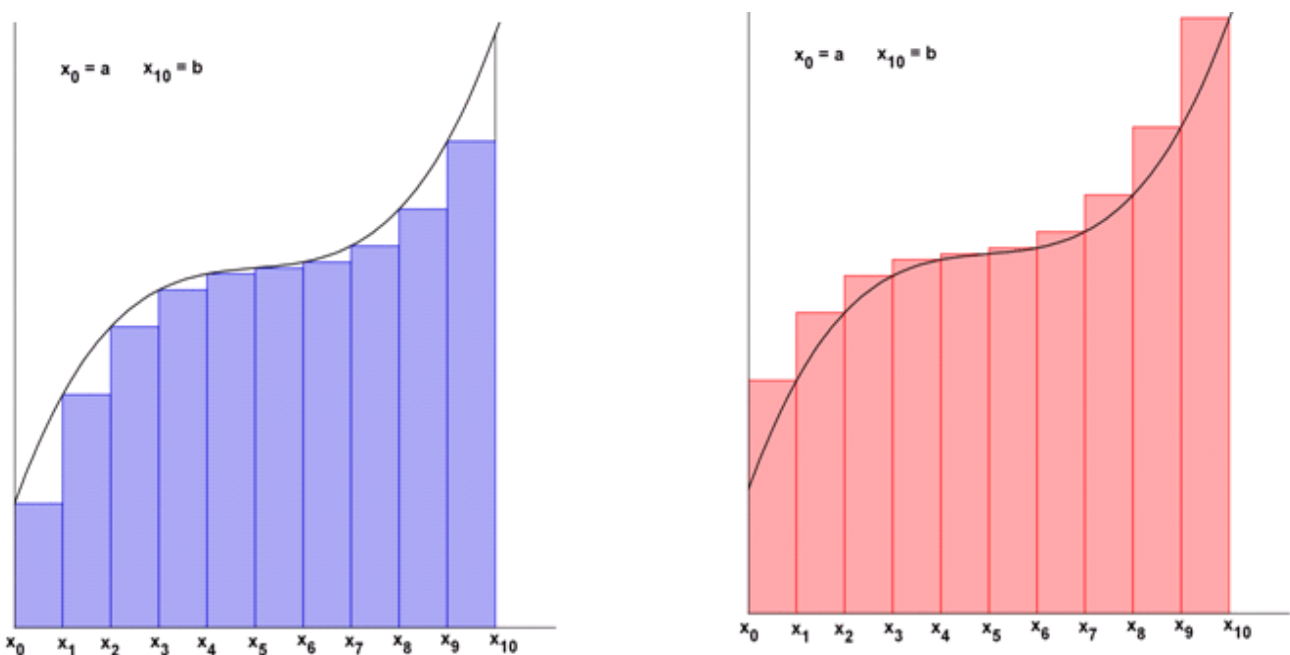
\includegraphics[width=0.8\linewidth]{Bilder/obersumme-untersumme} \\
		
		
		
		\begin{minipage}{0.45\linewidth}
		\textbf{Unter-Integral}		\\
		\\	
		$\underline{I} = \lim \limits_{d(Z) \rightarrow 0} \underline{US} $ \quad \textcolor{blue}{$\infty \cdot 0$} \\
		\\
		$\underline{I} =  \underline{\int \limits_{a}^{b}} f(x) \, dx $ \\
		
		\end{minipage}
		\hfill				
		\begin{minipage}{0.45\linewidth}
		
		
		\textbf{Ober-Integral}		\\
		\\	
		$\overline{I} = \lim \limits_{d(Z) \rightarrow 0} \overline{OS}$ \quad \textcolor{blue}{$\infty \cdot 0$} \\
		\\
		$\overline{I} =  \overline{\int \limits_{a}^{b}} f(x) \, dx $ \\

		\end{minipage}
		
		
		\subsubsection{Riemann-Summe S.506-507}
		RS = $\sum \limits_{i=0}^{n-1} f(\xi) \Delta x_i$  \quad $d(Z) \rightarrow 0 $ \quad $\int \limits_{a}^{b} f(x) \, dx$ \\
		\\
		$\xi \in [x_i ; x_{i+1}]$		
			
		
		\subsubsection{Riemann-Integral S.507}
		I = $\underline{I}$ = $\overline{I}$ wenn $\underline{I}$ = $\overline{I}$\\
		\\		
		\begin{minipage}{0.45\linewidth}
		Notation: $ \int \limits_{a}^{b} f(x)\, dx $
		\end{minipage}				
		\hfill
		\begin{minipage}{0.45\linewidth}
		\begin{tabular}{ll}
		$a$, $b$ & Integrationsgrenzen \\
		$f(x)$ & Integrand\\
		\end{tabular}
		\end{minipage}	
		
	
		
		\subsubsection{Integrierbare Funktionen}
		\textbf{Hinreichendes Kriterium: $f: [a;b] \rightarrow \mathbb{R}$ und $\mathbb{W}_f$ beschränkt}		 \\
		\\	
		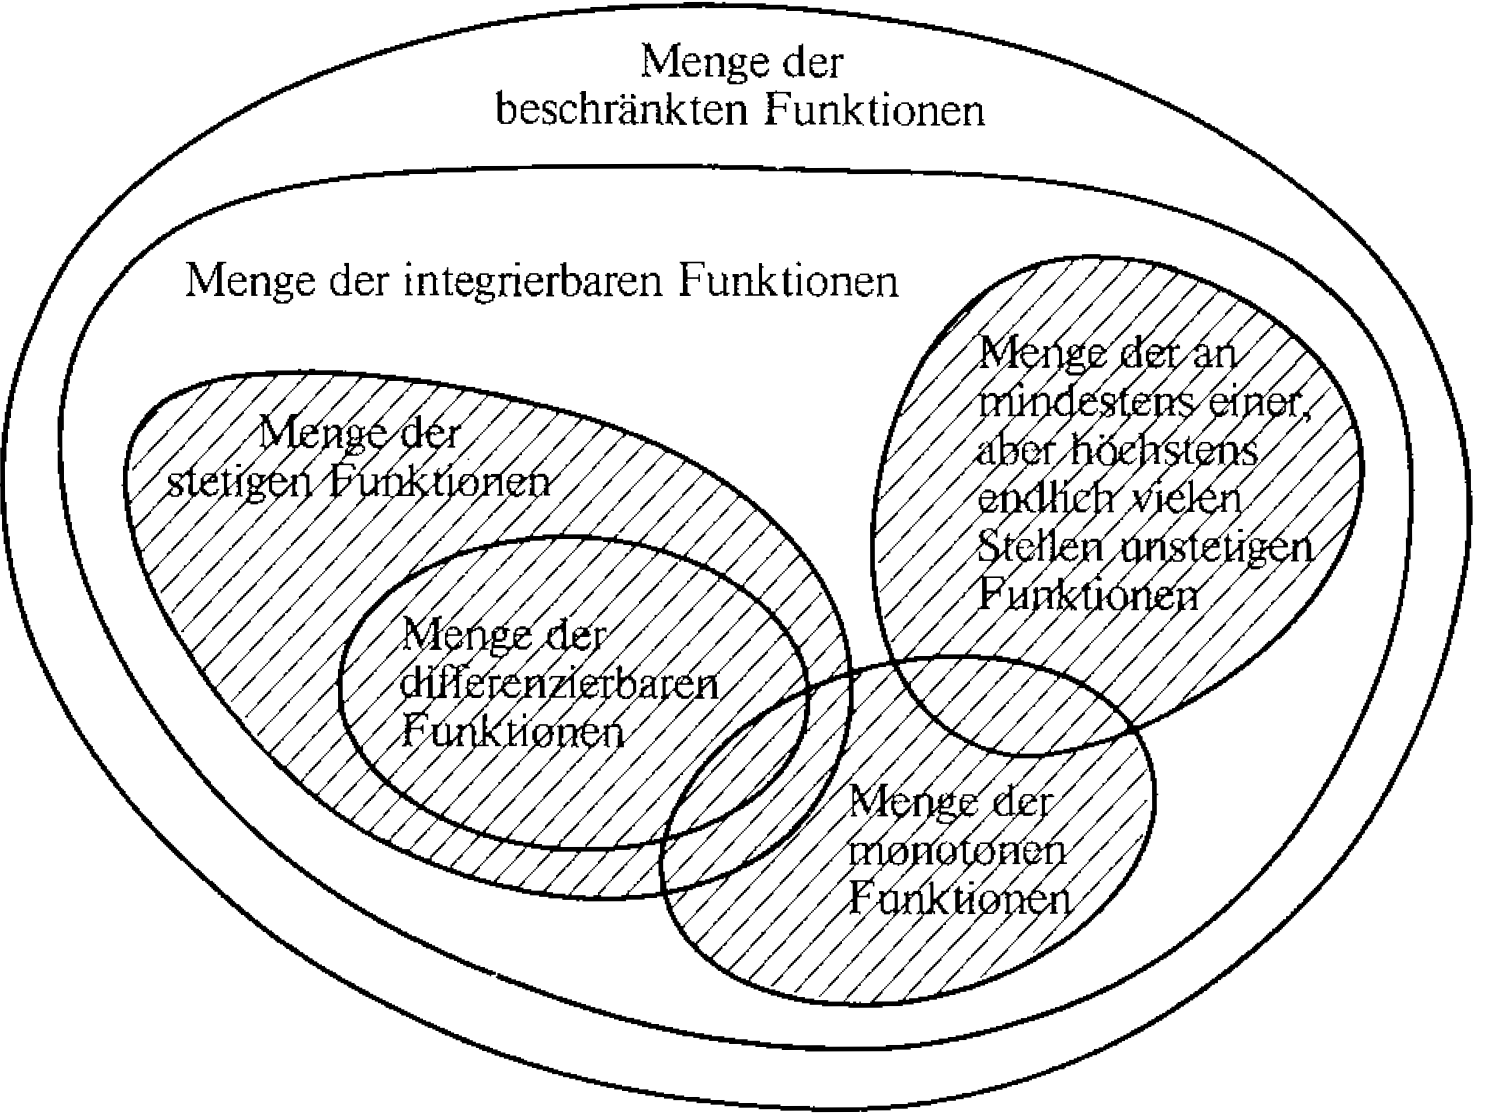
\includegraphics[width=0.7\linewidth]{Bilder/integrierbare-funktionen}
		
		
		\subsubsection{Integrationsregeln S. 494-496}
		Linearität: $\int \limits_{a}^{b} \alpha \, f(x) \, dx = \alpha \int \limits_{a}^{b} f(x)\, dx$ 
		
		
		\textbf{Rechenregeln mit Integralen S. 508-510}\\
		\begin{tabular}{ll}
		Zerlegung: & $\int \limits_{a}^{b} f_1(x) \, dx + f_2(x)\, dx = \int \limits_{a}^{b} f_1(x) \, dx + \int \limits_{a}^{b} f_2(x) \, dx$ \\
		\\		
		& $\int \limits_{a}^{c} f(x)\, dx = \int \limits_{a}^{b} f(x)\, dx + \int \limits_{b}^{c} f(x) \, dx$ \\
		\\
		Grenzen tauschen: & $ \int \limits_{a}^{b} f(x) \, dx = -  \int \limits_{b}^{a} f(x) \, dx $ \\
		\\
		Gleiche Grenzen: &  $\int \limits_{a}^{a} f(x) \, dx = 0$ \\
		\end{tabular}
		
		
		\subsubsection{Wichtige Integrale S. 495}
		\begin{tabular}{ll}
		$\int \limits_{a}^{b} x^2 \, dx = \frac{b^3}{3} - \frac{a^3}{3}$ & $\int \limits_{a}^{b} x \, dx = \frac{b^2}{2} - \frac{a^2}{2}$ \\
		\\
		$\int \limits_{a}^{b} 1 \, dx = b - a $ (Rechteck)& \\
		\end{tabular}
			
			
		\subsubsection{Flächen unter Integralen}
		\textbf{Voraussetzung: $f: [a;b] \rightarrow \mathbb{R}$ und $\mathbb{W}_f$ beschränkt}\\
		\\
		Fläche $A = \int \limits_{a}^{b} \vert f(x) \vert \, dx $ \\
		\\
		\textcolor{red}{Der Inhalt des Betrags muss auf Vorzeichen untersucht werden!} \\
		Negative Vorzeichen müssen über die x-Achse geklappt werden: \\
		$\vert x^2 - x \vert = -(x^2 - x)$ falls $x > x^2$ 
		
		
		\subsubsection{Mittelwert einer Funktion S. 510}		
		Funktion aufgeteilt in n äquidistante Intervalle $\rightarrow \Delta x = \frac{b-a}{n}$ \\
		\\
		Mittelwert: \quad $\frac{1}{b-a} \int \limits_{a}^{b} f(x) \, dx$
		
		
		\subsubsection{Mittelwertsatz S. 510}
			\textbf{Voraussetzung: $f: [a;b] \rightarrow \mathbb{R}$ und $\mathbb{W}_f$ beschränkt und stetig} \\
		Die Fläche unter der Funktion $f(x)$ kann an mind. einem Punkt $\xi$ als Rechteck dargestellt werden. \\
		$\xi \in (a;b)$ \\
			
		\begin{minipage}{0.40\linewidth}
		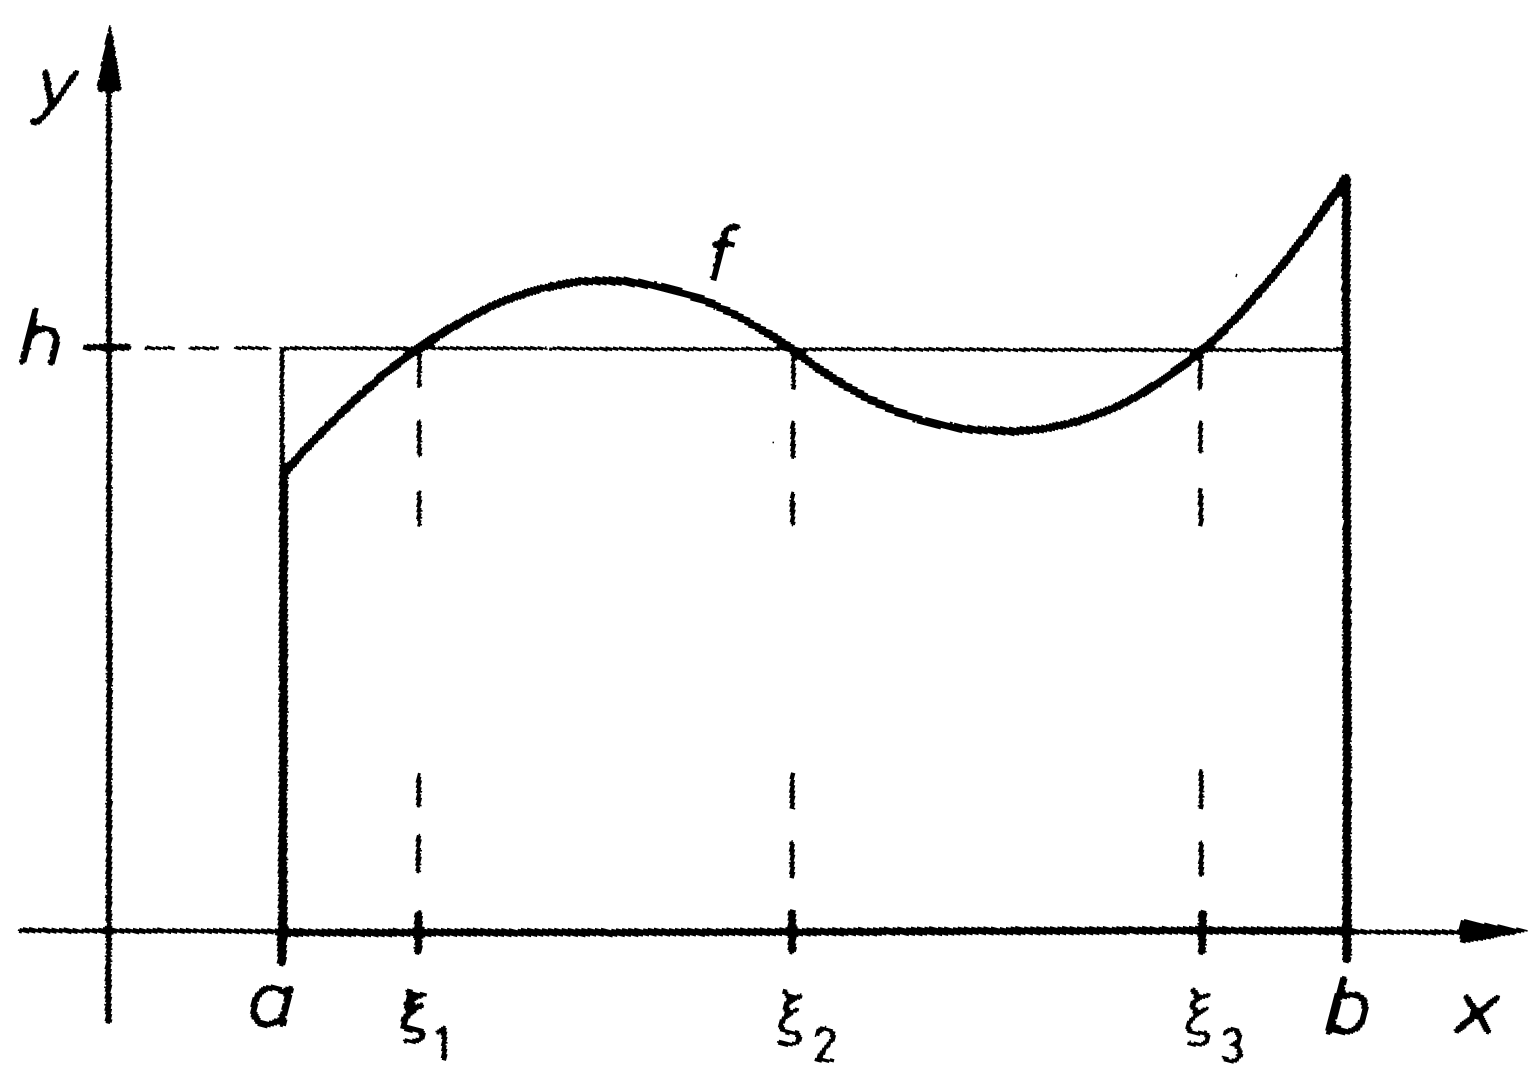
\includegraphics[width=0.95\linewidth]{Bilder/MWS-integral} \\
		\end{minipage}
		\hfill				
		\begin{minipage}{0.55\linewidth}
		
		Fläche =  Mittelwert $\cdot$ Intervall-Länge \\
		\\ 
		 $\frac{1}{b-a} \int \limits_{a}^{b} f(x) \, dx = f(\xi)$ \\
		$ \int \limits_{a}^{b} f(x) \, dx = (b-a) \cdot f(\xi)$ \\
		$ (b-a) \cdot h = (b-a) \cdot f(\xi)$ \\
		\end{minipage}
		
		
		\subsubsection{Integralfunktion I(x)}
		\textbf{Voraussetzung: $f: [a;b] \rightarrow \mathbb{R}$ und integrierbar} \\
		 \\
		 I(x) besitzt eine feste untere Grenze c = const (Anker) und eine variable obere Grenze x (Hauptvariable) \quad $x \in $[a;b] \qquad  $c \in $[a;b] \\
		 \\
		 Notation: $I(\tilde{x}) = \int \limits_{c}^{x} f(\tilde{x}) d\tilde{x} $  \qquad $\tilde{x}$ ist die Integrationsvariable 
		 
		 
		 \textbf{Eigenschaften der Integralfunktion}\\
			Die Integralfunktion hat beim Anker c eine Nullstelle: \\
			\\
			$I(c) = \int \limits_{c}^{c} f(\tilde{x}) \, d\tilde{x} = 0 $  \\
		\\	
		I(x) berührt/schneidet die x-Achse in [a;b] beim Anker \\
		$\rightarrow$ I(c) = 0 \\
		\\
		Das Verschieben des Ankers bewirkt eine Parallelverschiebung \\ 
		von I(x) \\
		
		\textbf{I(x) ist immer stetig!} (Integration behebt Sprungstellen) \\
		\textbf{I(x) ist ableitbar, \textcolor{red}{wenn die Originalfunktion f(x) stetig ist}}  \\
		\\
		Ableitung $I'(x) = \frac{d}{dx}\left( \int \limits_{c}^{x} f(\tilde{x}) \, d\tilde{x} \right) = f(x)$ \quad "Kreislauf" \\
		\\
		\\
		\begin{tabular}{l c l}
		Integral $I(x)$ &  $\underrightarrow{\text{differenzieren}}$ & $f(x)$ \\
		\\
		Integral $I(x)$ &  $\underleftarrow{\text{integrieren}}$ &  $f(x)$ 
		\end{tabular}
		
		
		\textbf{Beispiel Integralfunktion bestimmen}\\
		$f(x)=\left\{\begin{array}{ll} 1, & 0 \leq x < 0.75 \\
         -0.5, & 0.75 \leq x \leq 2 \end{array} \right.$	\\
     \\
     $I(x)=\left\{\begin{array}{l} \int \limits_{c=0}^{x} 1 \, d \tilde{x} = x \\
     \\
     \textcolor{red}{\int \limits_{c=0}^{0.75} 1 \, d \tilde{x}} + \int \limits_{0.75}^{x} (-0.5) \, d \tilde{x} = 0.75 + (-0.5)(x-0.75)\end{array} \right. $ \\
         	\\
         	\\
         	\textcolor{red}{Wichtig: Bei Funktionen mit Sprungstellen immer beim Anker \\
         	beginnnen, wenn nichts spezielles verlangt ist} \\
         	
		\subsubsection{Stammfunktion F}
		Eine Funktion $F(x)$ heisst Stammfunktion von $f(x)$ wenn gilt: \\
		\textbf{F'(x) = f(x)} \\
		\\
		$F(x) + C$ sind ebenfalls Stammfunktionen von $f(x)$ \\
		$C \in \mathbb{R}$ \quad C ist eine freie Verschiebungszahl\\
		\\
		Stammfunktionen $F$ sind Teilmenge der unbestimmten Integrale\\
		\\
		$\Rightarrow$ Ableitungstabelle rückwärts lesen für Stammfunktion!
		
		
		\subsubsection{Unbestimmtes Integral}
			$I(x) + C = \int \limits f(\tilde{x}) \, d\tilde{x} $ \quad  $C \in \mathbb{R}$ \\
			\\
			\textbf{Wenn $f(x)$ stetig ist, dann entspricht das unbestimmte Integral der Stammfunktion}
		
		
		\subsubsection{Hauptsatz der Integration S. 507}
		$\int \limits_a^b f(x) \, dx = F(b) - F(a) = \left[ F(x) \right]_a^b = F(x) \vert_a^b $
			
	
	
	\subsubsection{Wachstumsvergleiche}			 
			\begin{tabular}{llll}
			(1) & $\frac{n^k}{q^n} (n \rightarrow \infty)= 0$  & (k $\in \mathbb{N}; q > 1)$ & $\frac{\text{Potenz}}{\text{Exponentiell}} \rightarrow 0$\\
			\\
			(2) & $\frac{q^n}{n!} (n \rightarrow \infty)= 0$ & $(q > 1)$ & $\frac{\text{Exponentiell}}{\text{Fakult"at}} \rightarrow 0$ \\
			\\
			(3) & $\frac{\ln(n)}{n^k} (n \rightarrow \infty)= 0$ & (k $\in \mathbb{N})$ & $\frac{\text{Logarithmisch}}{\text{Potenz}} \rightarrow 0$ \\
			\\
			(4) & $\frac{\ln(n)}{n} (n \rightarrow \infty)= 0$ & & $\frac{\text{Logarithmisch}}{\text{Linear}} \rightarrow 0$ \\
			\end{tabular}